
% Section: EVALUATION
%\subsection{Performance Evaluation}
\subsection{Evaluation}
\label{sec__bandwidth_truthfulness_evaluation}

We conduct the simulation experiments using the multi-agent programmable modelling environment NetLogo \cite{Wilensky1999NetLogo}.
In all the experiments, we consider a single provider and 500 users.
We run the experiments for 1000 rounds, and plot the average values in the graphs.

For different pricing mechanisms (as explained in \cref{sec:model-pricing}), we use the following values.
	For fixed pricing, we set $c_0 = 0.5$.
	For priority pricing, we set $c_{h_0} = 0.25$ and $c_{h_1} = 0.75$.
	For auctions based pricing, the bids for lower priority requests $h_0$ are uniformly distributed in the range $[0.25, 0.5]$, 
	while the bids for higher priority requests $h_1$ are uniformly distributed in the range $(0.5, 0.75]$.
For differentiating between the two priority classes, we choose different time-utility functions (TUF), 
which in this case we have chosen as step functions for simplicity.
According to this step function, the value $v_i(h, t)$, based on priority class $h$ and slot $t$ in schedule $\phi$, 
decreases for both higher and lower priority classes after a threshold $t_0 = \frac{N}{2}$, as shown in Figure~\ref{fig:value_fn}. 
Specifically, for lower priority class $h_0$:
%
\begin{equation}
	v_i(h_0, t) = 
		\begin{cases}
		1.5 &	\text{if }	t \leq \frac{N}{2}  \\
		1 &	\text{if }	\frac{N}{2} < t \leq N
		\end{cases}
\end{equation}
%
And for high priority class $h_1$:
\begin{equation}
	v_i(h_1, t) = 
		\begin{cases}
		3 &	\text{if }	t \leq \frac{N}{2}  \\
		2 &	\text{if }	\frac{N}{2} < t \leq N
		\end{cases}
\end{equation}


%% FIGURE
\begin{figure}[tbp]
	\centering
	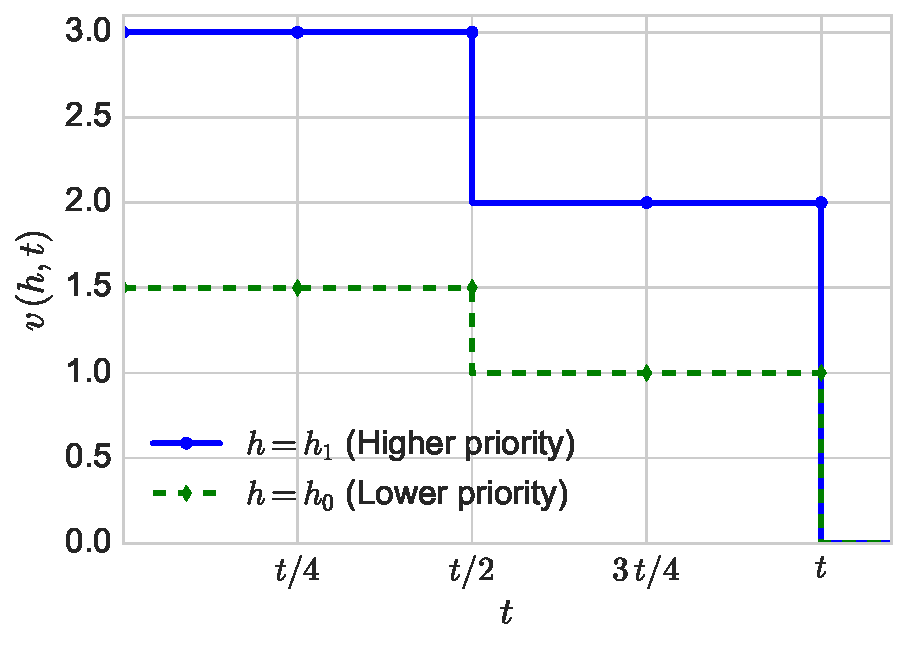
\includegraphics[width=0.65\columnwidth,keepaspectratio]{value-fn}
	\caption[Value function $v_i(h, t)$ for user $i$]{Value function $v_i(h, t)$ for user $i$ based on priority class $h$ and slot $t$ in schedule}
	\label{fig:value_fn}
\end{figure} 


Each user $i$ submits exactly one request to $\mathcal{P}$, declaring her priority class $h_i$, value $v_i$, and bid amount $b_i$ where applicable.
Both the priority classes, $h_0$ and $h_1$ occur with the same probability, so almost half of the requests are of higher priority, and the rest are of lower priority. 
We model lying behaviour of the users, by randomly flipping their reported priority class $h$ to $\mathcal{P}$, according to a uniform distribution.
When the users lie, we observe the normalised difference from the case where all the users are truthful.
Here, $u^*_i(\phi,t)$ indicates the case where the users lie to $\mathcal{P}$,
and $u_i(\phi,t)$ where all the users are truthful.

\begin{equation}
	\Delta \ \textrm{\itshape welfare} = \frac{
						\displaystyle\sum_{i \in N} u^*_i(\phi,t) - 
						\displaystyle\sum_{i \in N} u_i(\phi,t)
					}{
						\displaystyle\sum_{i \in N} u_i(\phi,t)
					}
\end{equation}

\subsubsection{Social Welfare}
Figure~\ref{fig__welfare_vs_liars} shows how social welfare is affected when the probability $p\,(lying)$ of a user misreporting her value to 
$\mathcal{P}$ increases up to the point where 90\% of the users may be lying.
As expected, social welfare decreases as the probability of lying increases, since $\mathcal{P}$ fails to allocate better slots for higher priority requests.
All the pricing schemes behave similarly as the proportion of lying users increases, 
except VCG which performs marginally better in that social welfare is slightly higher for VCG as compared to the other schemes.
This shows the importance of encouraging truthful behaviour in the users for maximising social welfare.

\begin{figure}[tbp]
	\centering
	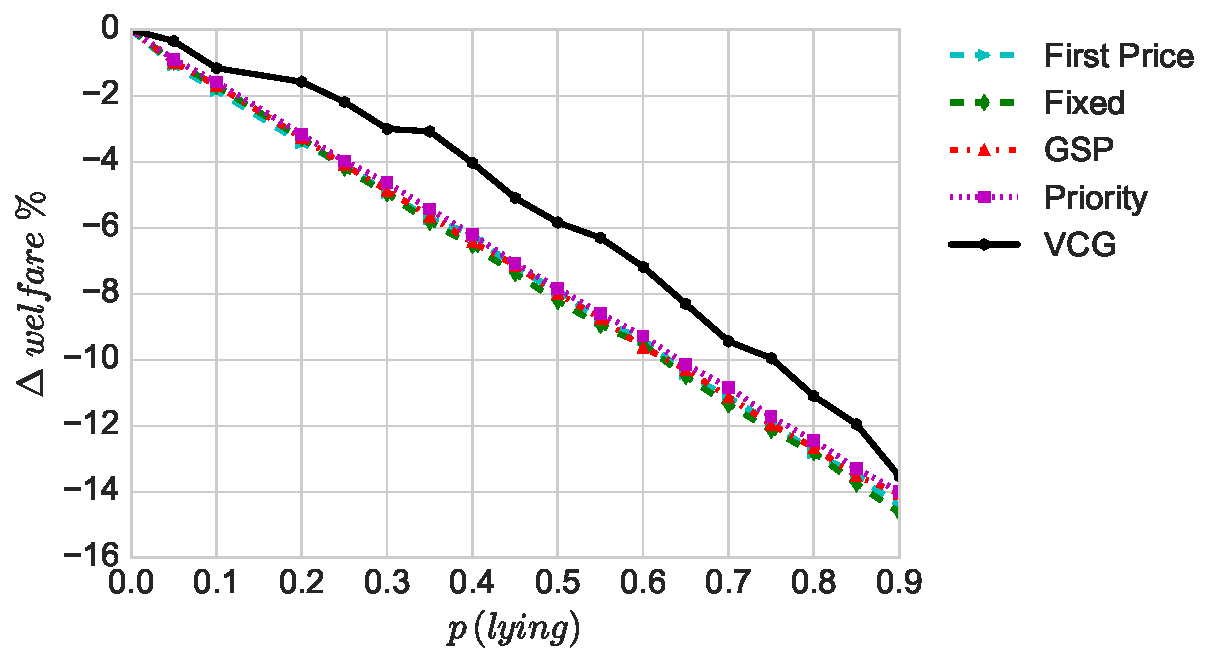
\includegraphics[width=0.75\textwidth,keepaspectratio]{welfare_vs_liars}
	\caption{Percentage difference in social welfare as more users lie}
	\label{fig__welfare_vs_liars}
\end{figure}

\subsubsection{Individual Gain in Utility for Different Classes}
To understand how the pricing mechanisms incentivise truthfulness for different priority classes, 
in the next experiment we look at the normalised difference in utility for an individual user (on average), separately for $h_0$ and $h_1$.
Here again, $u^*_i(\phi,t)$ is the individual utility when some of the users lie,
and $u_i(\phi,t)$ is when all the users are truthful.

\begin{equation}
	\Delta \ \textrm{\itshape utility} = \frac{
						u^*_i(\phi,t) - 
						u_i(\phi,t)
					}{
						u_i(\phi,t)
					}
\end{equation}


Figure~\ref{fig__util_low_vs_liars} shows the percentage difference in the average utility for all the users with low priority requests.
Note that this average is over all the users in $h_0$, and not only those who lie.
Users from $h_0$ may lie in order to get higher value (through reserving an earlier slot),
hoping to still pay as little as possible. 
Figure~\ref{fig__util_low_vs_liars} shows that for fixed usage-based price, they do gain in utility since they are paying the same amount for a better service.
For priority pricing, they gain nothing as any gains in utility are offset by the higher price.
For first price and GSP auctions, the results are similar and there are gains due to lying, though less than those in the case of the fixed price.
The first price and GSP auctions behave similarly since expected payments are the same in the first and second price auctions, when the bids are independent and identically distributed~\cite{Maille2014}, as is the case in this experiment. 
VCG performs better since the utility decreases as more users lie.

\begin{figure}[tbp]
	\centering
	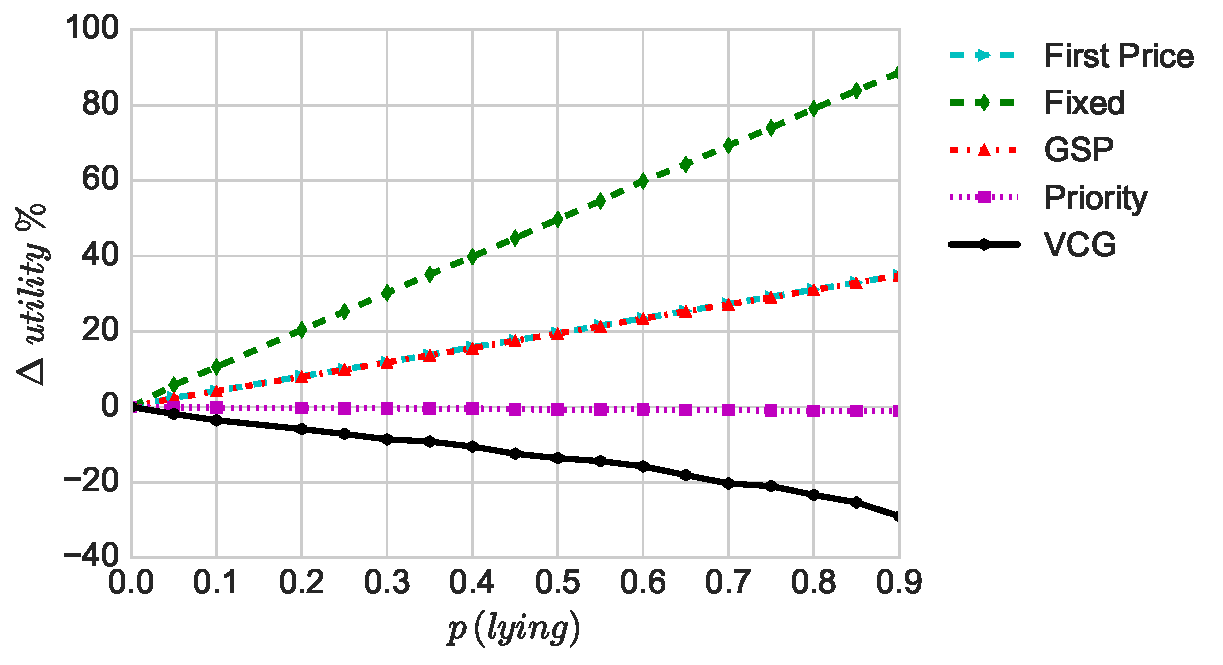
\includegraphics[width=0.75\textwidth,keepaspectratio]{util_low_vs_liars}
	\caption{Percentage difference in utility for low priority class $h_0$}
	\label{fig__util_low_vs_liars}
\end{figure}

Figure~\ref{fig__util_high_vs_liars} shows the percentage difference in the average utility for all the users with high priority requests.
Note that this average is over all the users in $h_1$, and not only those who lie.
Users from $h_1$ may lie in order to save on their payments, with the hope that they can still get the same value (through keeping their earlier slot). 
Figure~\ref{fig__util_low_vs_liars} shows that users from $h_1$, in general, lose by lying since there is little chance that $\mathcal{P}$ will assign earlier slots to the users declaring low priority to $\mathcal{P}$.
So even though they save on the payments, the decrease in value because of getting assigned later slots results in net loss for users from $h_1$.

\begin{figure}[tbp]
	\centering
	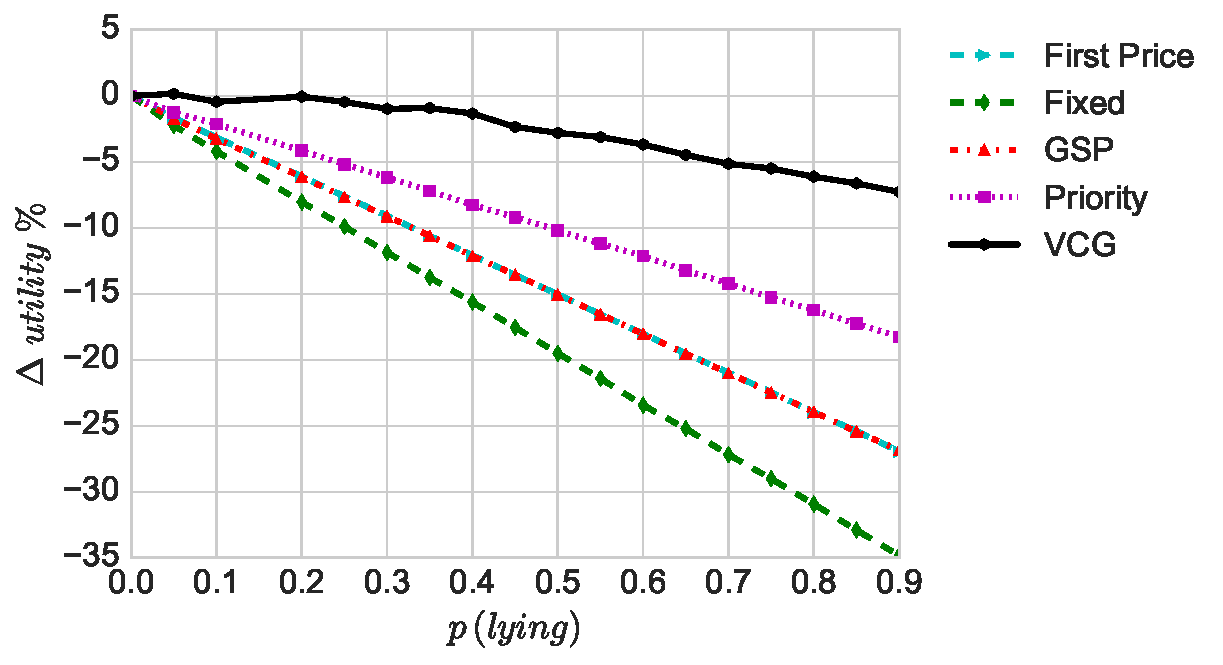
\includegraphics[width=0.75\textwidth,keepaspectratio]{util_high_vs_liars}
	\caption{Percentage difference in utility for high priority class $h_1$}
	\label{fig__util_high_vs_liars}
\end{figure}

\subsubsection{Maximum Gains}
In the next experiment, we look specifically at the utility for the users that report untruthful values to $\mathcal{P}$,
to see the maximum gain they can get in the utility under different pricing mechanisms.
Figure~\ref{fig__util_low_max_by_lying} shows the maximum gain in utility a user from $h_0$ can get as the number of lying users increases.
Note that in this case we pick only the maximum utility for a user from $h_0$ that is lying, averaged across all the experiment runs.
The results are similar to what we observed earlier in Figure~\ref{fig__util_low_vs_liars}.

\begin{figure}[tbp]
	\centering
	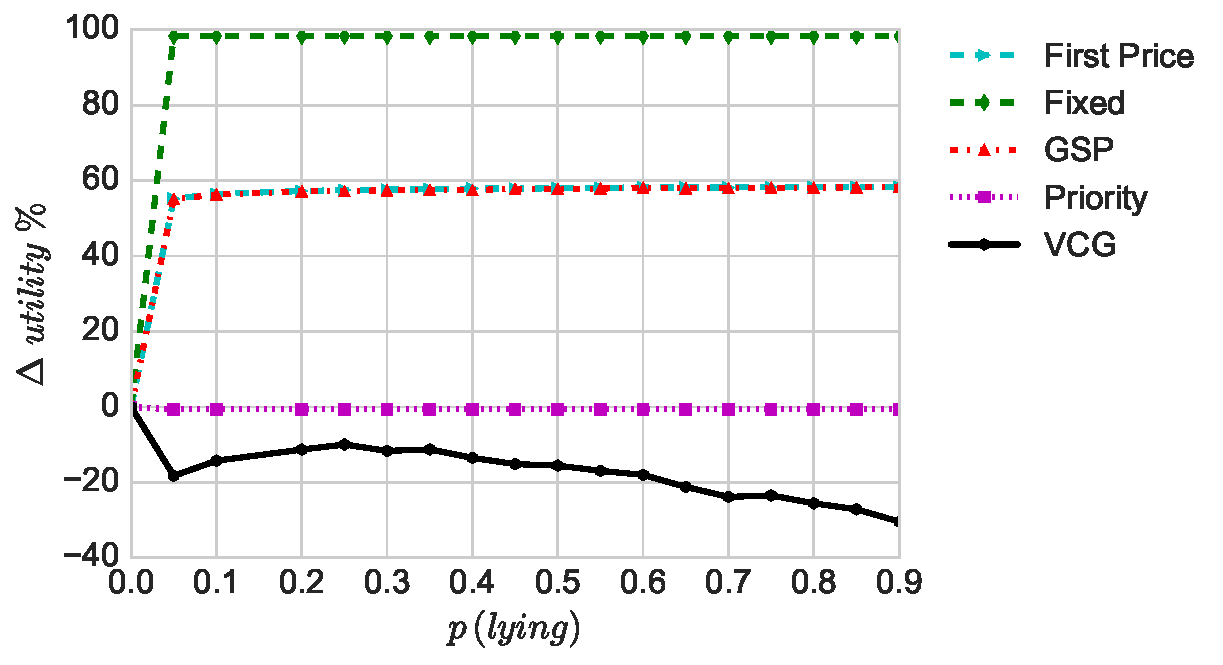
\includegraphics[width=0.75\textwidth,keepaspectratio]{util_low_max_by_lying}
	\caption{Maximum gain in utility for a user from low priority class $h_0$}
	\label{fig__util_low_max_by_lying}
\end{figure}

Similarly, Figure~\ref{fig__util_high_max_by_lying} shows the maximum gain in utility a user from $h_1$ can obtain through lying.
We noticed in Figure~\ref{fig__util_high_vs_liars} that on average the users from $h_1$ do not gain through lying,
but here we see that for all the pricing mechanisms except VCG, the utility for a lying user with high priority request increases with increase in the number of lying users, though the net gain is not significant.
For VCG, the number of lying users does not have much impact, and the loss in utility for the lying user remains almost the same.
Moreover, first price and GSP auctions perform better than priority pricing here.
The user can have a net gain in utility by misreporting her priority class as $h_0$ when more than half of the users are lying in the case of priority pricing.

\begin{figure}[tbp]
	\centering
	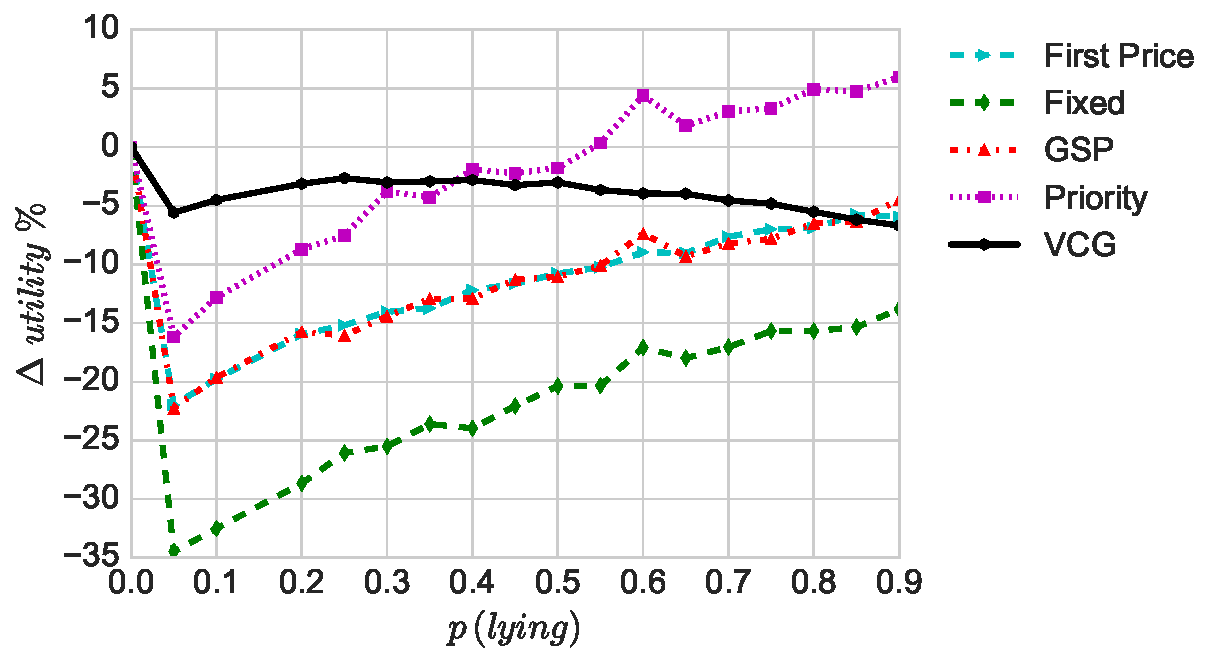
\includegraphics[width=0.75\textwidth,keepaspectratio]{util_high_max_by_lying}
	\caption{Maximum gain in utility for a user from high priority class $h_1$}
	\label{fig__util_high_max_by_lying}
\end{figure}

